% Experiments

\chapter{Experimentation}
In this chapter, we will go through the process, result and analysis of two experiments for Voxer's comparative testing in Keravan Energy's cooling system. The pressure meter used in both tests is Danfoss PFM 100 \cite{danfoss:web} which measures Kv factor, pressure and flow rate. All of equipments and components needed for operation are mentioned in appendix. The CAD models for pipeline and source code for analysis are also presented in appendix. Figure \vref{fig:orgpipe} shows the original cooling piping section in Keravan Energy. The pipeline includes these main components: one 5 meters of straight pipe, two 90 degree curves and rubber hoses.
\begin{figure}[h]
  \centering
  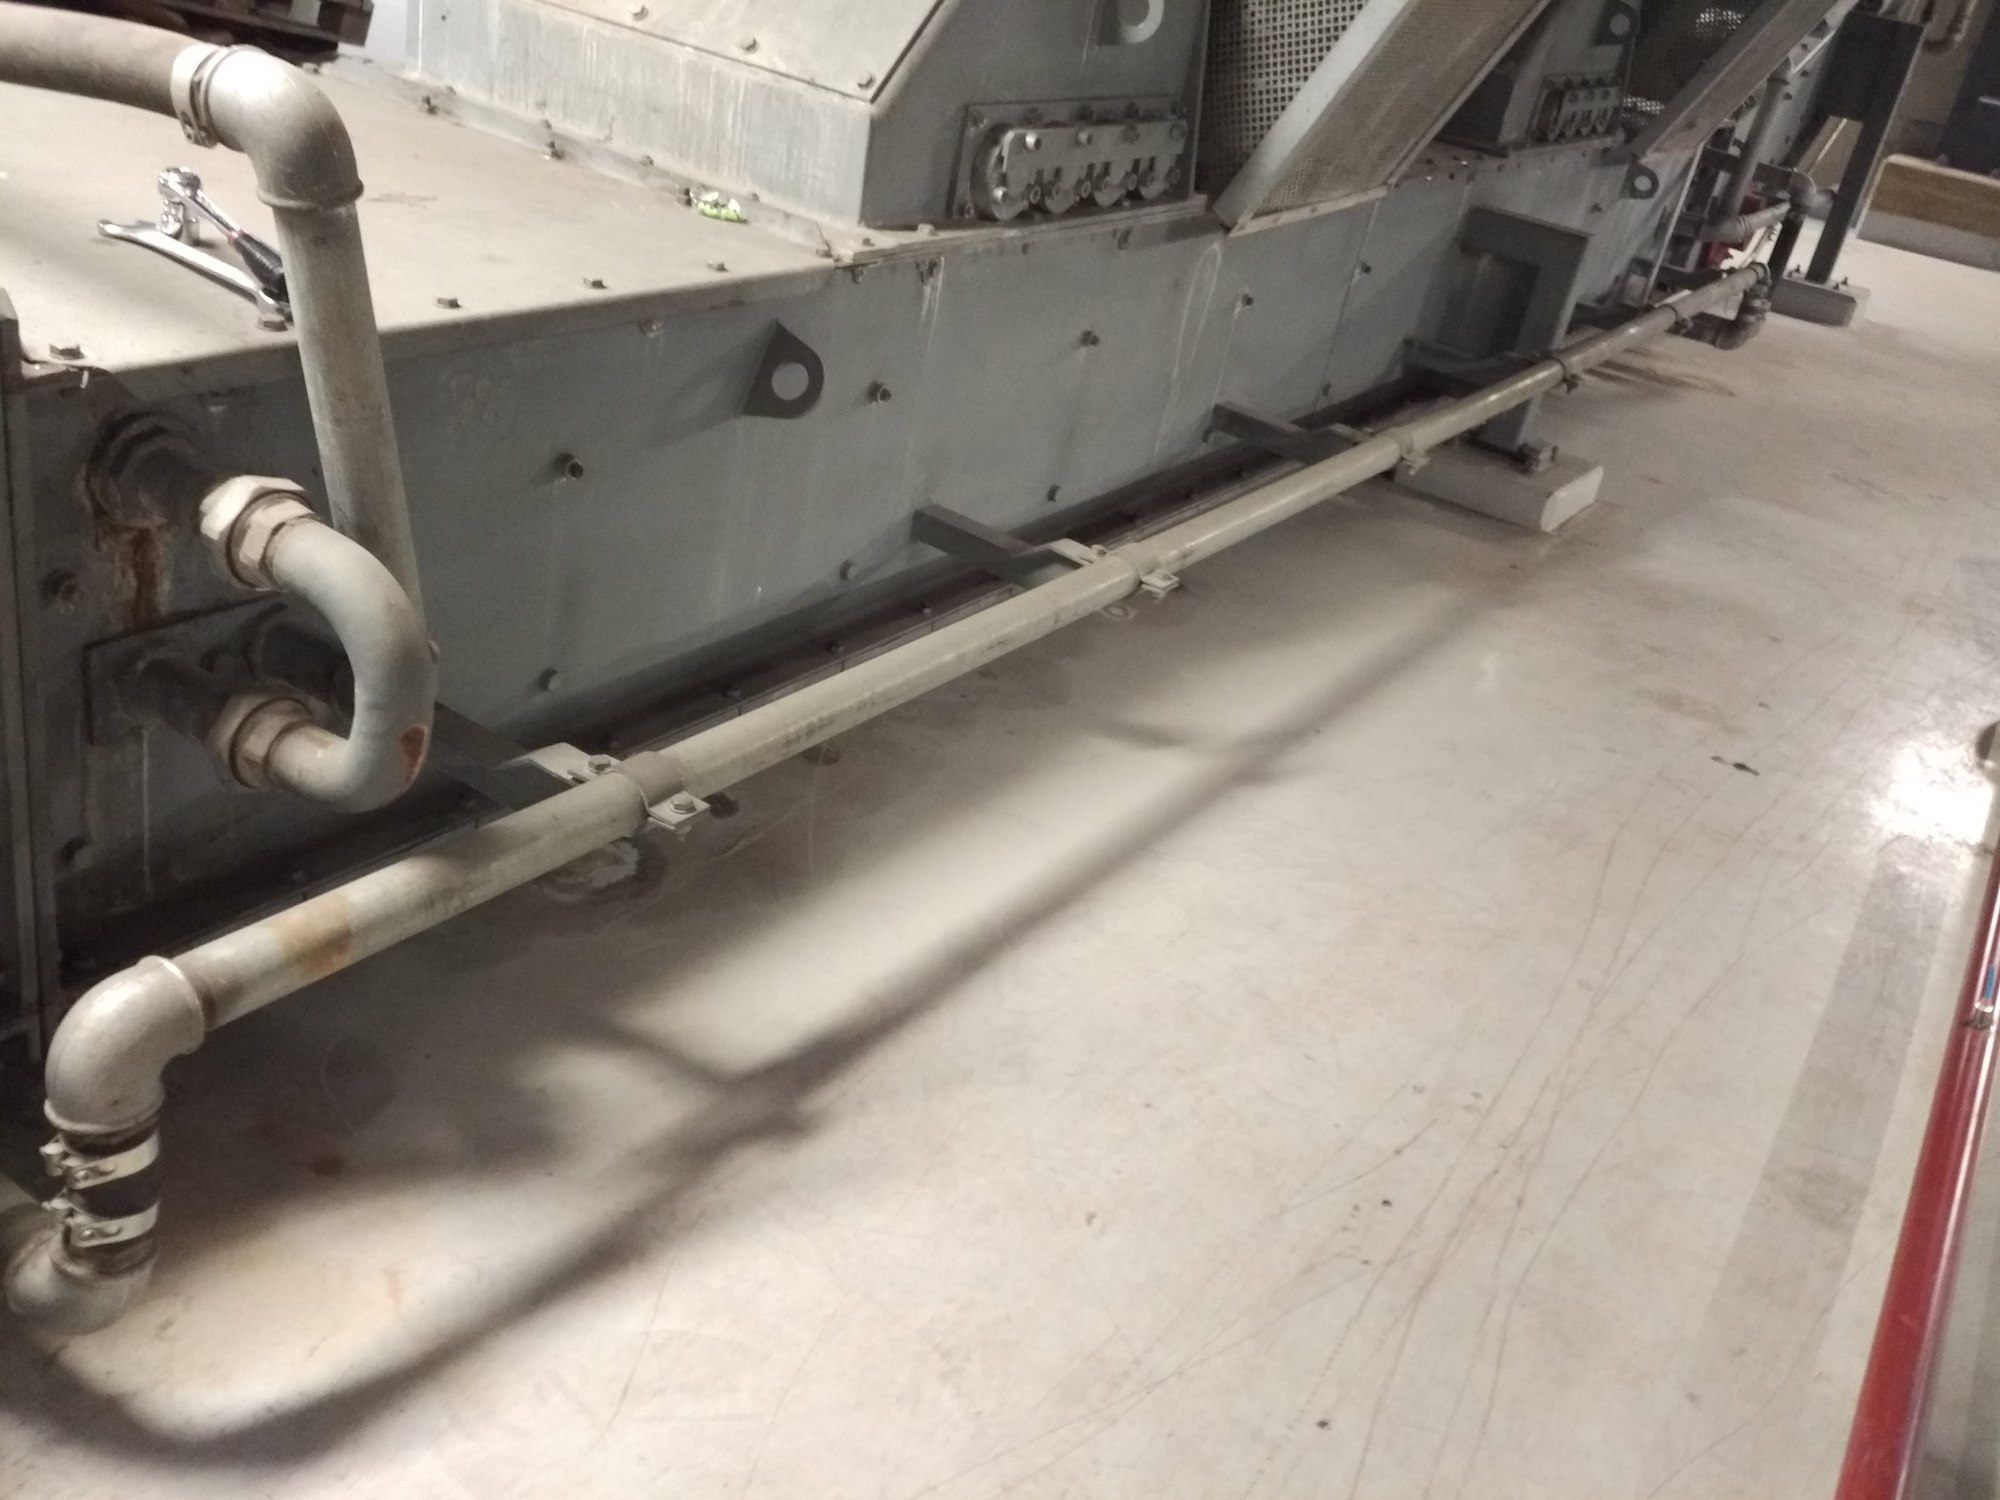
\includegraphics[width=8cm]{original_pipe}
  \caption{ Targeted piping system in Keravan Energy}
  \label{fig:orgpipe}
\end{figure}
\section{Laboratory experimentation}
It is essential to get a full understanding about the hydraulic system, product testing and objectives. In order to achieve this, it is advised to perform comparative measurements under laboratory condition first. In this setting, we will acquire more knowledge about factors which could affect to the system, proper techniques, required conditions and practices which needed to be applied to ensure the quality of measurement. Moreover, the data acquired would be more stable under controlled setting.
\subsection{Experiment's design}
The main goal of this laboratory experimentation is setting up the closest replication of cooling piping section with PP material and determining which Voxer combination is the best for the real test in Keravan Energy. Apart from that, there are some other learning points in this test also; for example: understanding the structure of the targeted pipeline, learning about Voxer and how to assemble it into the system, insights from impacts of different setting conditions to the result of measurements.
\begin{figure}[h]
  \centering
  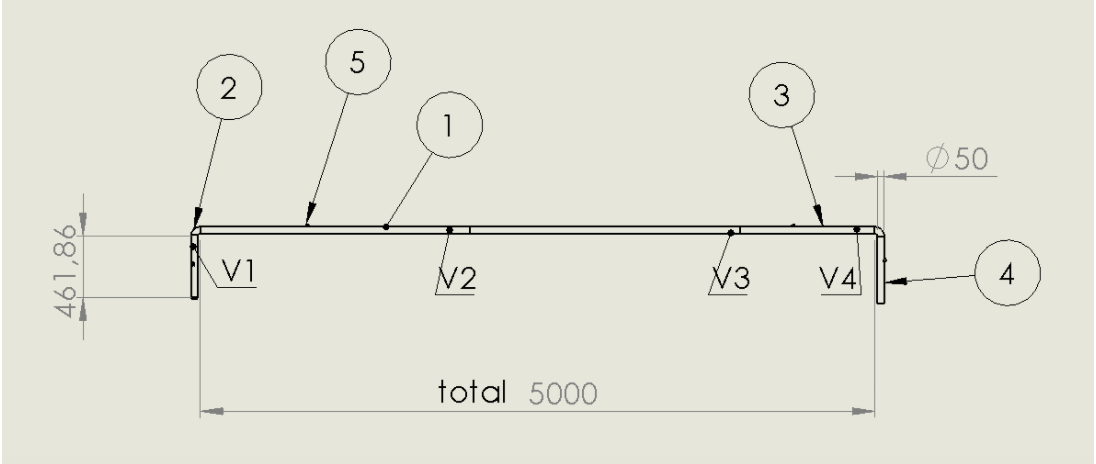
\includegraphics[width=8cm]{cadlab}
  \caption{ Basic pipe layout and positions of measuring points and Voxer wings \newline 1) Straight pipes 2 m; 2) 90 degree curves; 3) Straight pipe 1 m; 4) Straight pipe 0.5 m; 5) Plane connectors for measuring points}
  \label{fig:cadlab}
\end{figure}
Figure \vref{fig:cadlab} illustrated the basic setting of the pipelines. There are 4 measuring points which associates with plane connectors. The reason for creating these connectors is to create flat surface for ensuring secured pressurization of measuring points. It also minimizes the interference of the measuring device to the pressure and flow in the system. Each Voxer is connected to the end of each straight pipe, except the last one. There are maximum 4 Voxers using in each of measurement. With this settings, the pipeline is divided into 3 sections as pipes in series where total pressure is the accumulation of pressure from each section of the whole pipeline. In this experiment, we named section A from point 1 to 2, section B from point 2 to 3 and section C from point 3 to 4. Section T indicates the whole pipe from point 1 to 4 as the beginning and the end of the system. 
Since pipes are connected in series, we have:
\begin{align}
\delta P_t&= P_a + P_b + P_c = P_ab + P_c \\
\delta P_t&= \tn{Total pressure change in pipeline} \\
P_a&= \tn{Pressure change in section A} \\
P_b&= \tn{Pressure change in section B} \\
P_c&= \tn{Pressure change in section C} \\
P_ab&= \tn{Pressure change in section A and B} \\
\end{align}
There are 2 types of Voxer which were used in the test :Voxer 40 degree DN40 and Voxer 30 degree DN40.  Different combinations of the amount of Voxer and types of Voxer were carried out to determine the behavior of flow in each section and find out the best combination. Table \ref{table:combi} lists out the combinations performed in this test. The pressure changes between section A, section A and B and total pipe were measured in every combination. Every measurement was repeated 10 times to ensure balanced values. During the test, the average temperature of water in vessel was measured also to consider its influence on fluid viscosity and surface tension.
\begin{table}[h]
  \centering
  \caption{Voxer combination in lab test.\newline (V1 : Voxer in pipe 1; V12: Voxers in pipe 1 and 2, etc)}
  \begin{tabular}{l*{6}{c}}
Type             & V0 & V1 & V12 & V123 & V1234 & V14 \\
\hline
None & X & - & - & - & - & -   \\
30 degree           & - & X & X & X &  X & X  \\
40 degree           & - & X & X & X &  X & X   \\
Mixed     & - & - & - & - & - & X   \\
\end{tabular}
  \label{table:combi}
\end{table}
\subsection{Setting of experiments}
\textbf{Main pipe} \newline
The pipeline test system was set like firgure \vref{fig:cadlab} in Metropolia’s laboratory.  Pipes were connected with others in series. The main straight horizontal pipe section is 5 meters long in total, which included two 2 meters of straight pipes and one 1 meter of straight pipe. Each side of main straight pipe was fitted with a 90 degree curve. There were two 0.5 meters of vertical pipe extensions at each side, acting as extended pipes for placing Voxer and measuring points. Two reducers were attached with these extended in order to accommodate the hose pump. Figure \vref{fig:wholepipe} demonstrates the completed setting of pipe.
\begin{figure}[h]
  \centering
  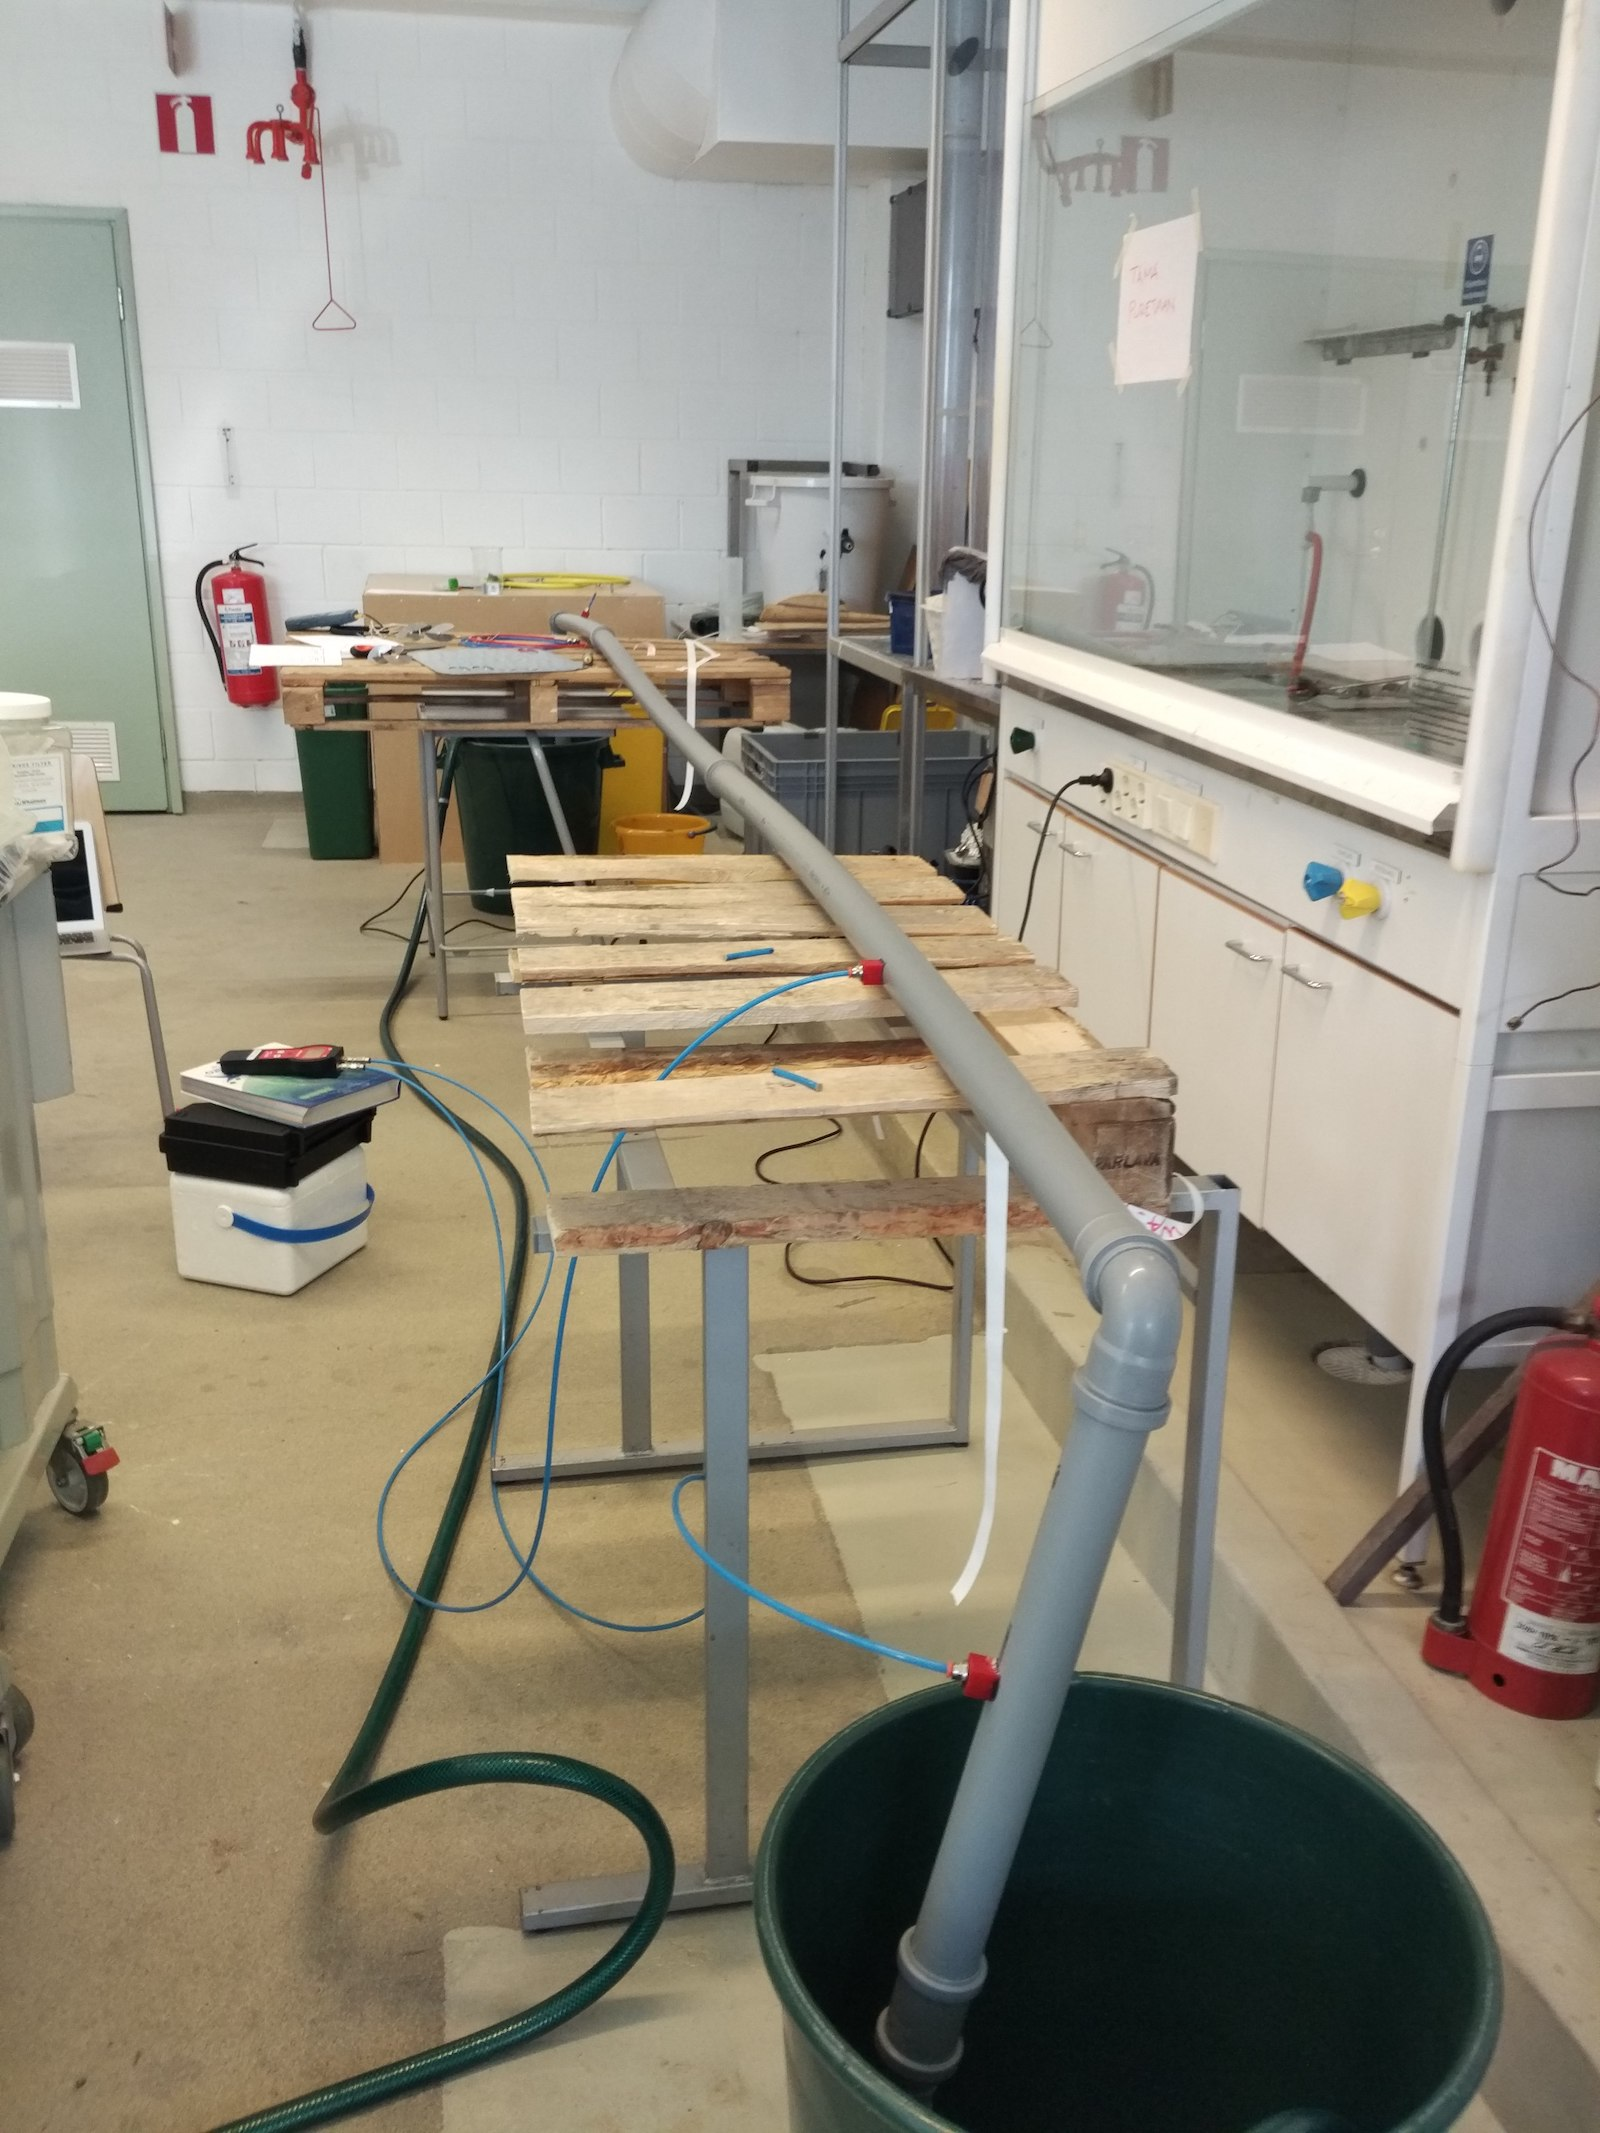
\includegraphics[width=8cm]{wholepipe}
  \caption{View of the whole test pipeline in Metropolia's lab }
  \label{fig:wholepipe}
\end{figure}

\textbf{Connectors, pump and vessels}\newline
Pressure meter’s hoses were attached to the pipe by 4 plastic plane connectors glued above small holes on the pipe (see figure \vref{fig:connector}). Voxers were separated from metal sheet, bended and twisted following given instruction from SansOx Ltd. and inserted into different positions of the pipeline (see firgure \vref{fig:vox}). As mentioned before, the positions of Voxer were mainly at the end of each pipe. The system was set above the ground with 2 vessels at each side to keep the flow going with gravity, one as water reservoir and one for precaution leaking. A pump was positioned in water reservoir and connected with the starting pipe by hose. Water was delivered through the system and come back to the water reservoir. The ending pipe was submerged completely into water to balance static pressure in the system (see figure \vref{fig:subpipe}).

\begin{figure}[!htb]
   \begin{minipage}{0.48\textwidth}
     \centering
     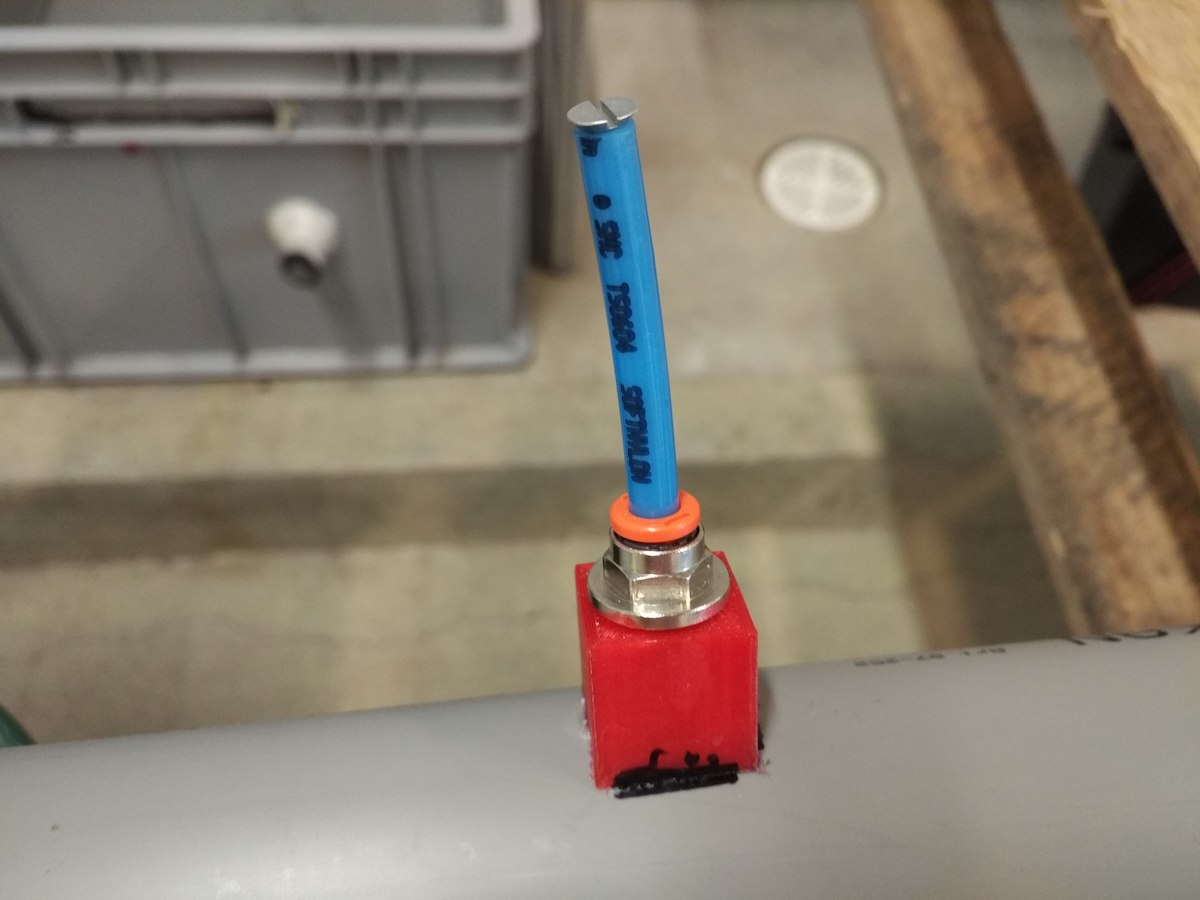
\includegraphics[width=0.9\linewidth]{connector}
     \caption{Connector as measuring points}\label{fig:connector}
   \end{minipage}\hfill
   \begin {minipage}{0.48\textwidth}
     \centering
     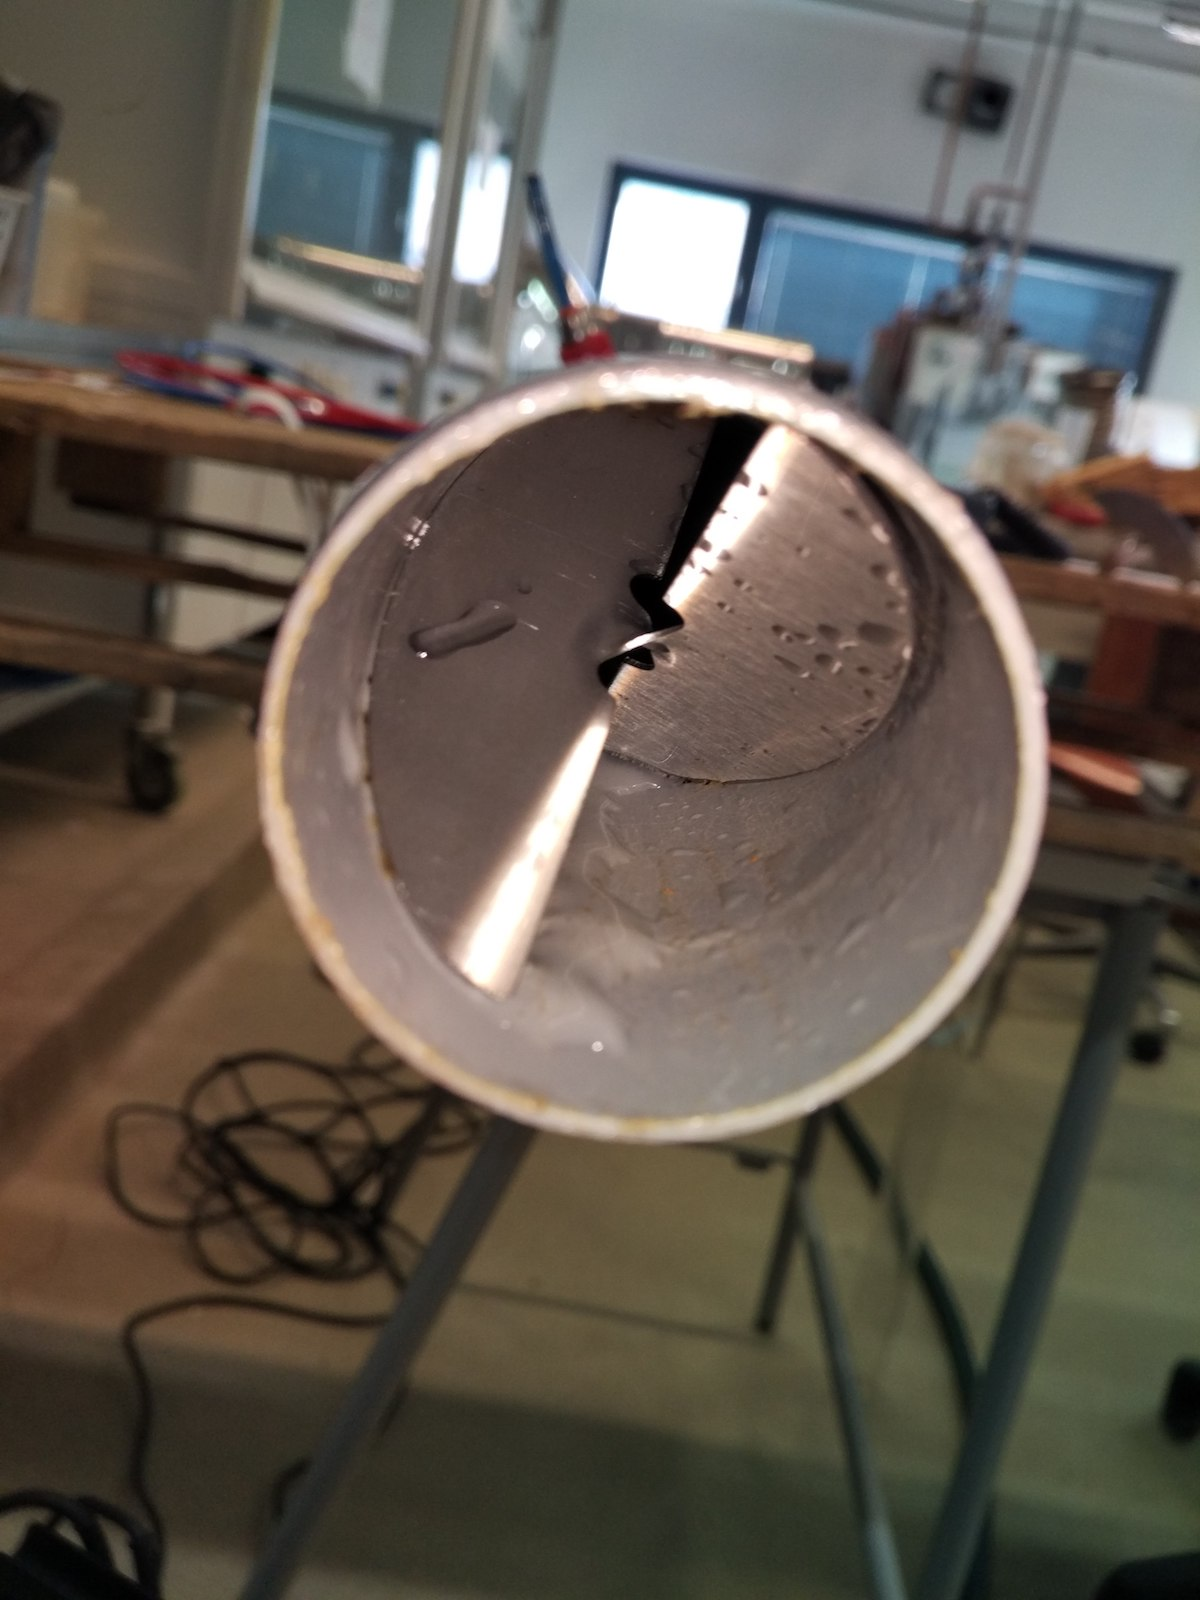
\includegraphics[width=.6\linewidth]{vox}
     \caption{Voxer wing inside pipe}\label{fig:vox}
   \end{minipage}
\end{figure}
\begin{figure}[h]
  \centering
  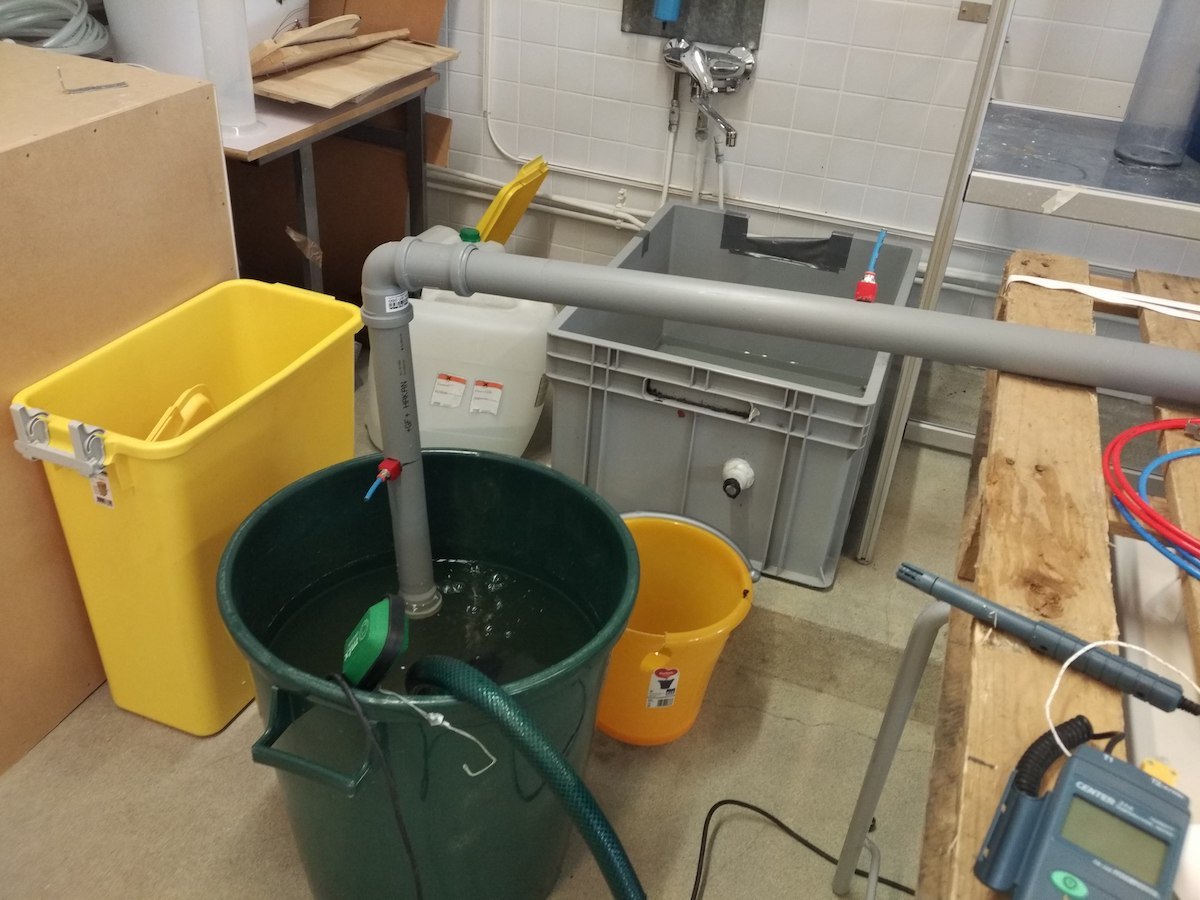
\includegraphics[width=9cm]{sub-pipe}
  \caption{ The ending pipe was submerged into water in reservoir}
  \label{fig:subpipe}
\end{figure}
\subsection{Result and analysis}
The data acquired from the lab experiment is treated 
\section{Experimentation in Keravan Energy}
\subsection{Experiment's design}
\subsection{Setting of experiments}
\subsection{Result and analysis}

\clearpage %force the next chapter to start on a new page. Keep that as the last line of your chapter!
